
%!TEX TS-program = xelatex
%!TEX encoding = UTF-8 Unicode

\documentclass[12pt]{article}
\usepackage{geometry}                
\geometry{letterpaper}                   
\usepackage{amsmath}
\usepackage{graphicx}
\usepackage{amssymb}
\usepackage{tikz}
\usepackage{framed}
\usepackage{listings}
\lstset{language=Octave,
  basicstyle=\footnotesize,
  tabsize=3,
  breaklines=true,
  mathescape=true,
  commentstyle=\color{blue},
  morecomment=[l]{\#}}



\author{Elliott Hauser}
\title{Comp 555 Problem Set 4}
\begin{document}
\maketitle

\section*{Question 1}
1. Consider the following four sequences 
Chimp GTTG
Gorilla  GTCA
Human  ACCA
Orangutan ATTA
Assume the following scoring matrix
  A T G C
A 0 2 3 8
T 2 0 1 3
G 3 1 0 3
C 8 3 3 0

\paragraph{a.} % (fold)
\label{par:1a}
Six binary tree topologies with two different tree structures are shown in Figure~\ref{trees}. 

\begin{figure}[htb]
	\begin{center}
		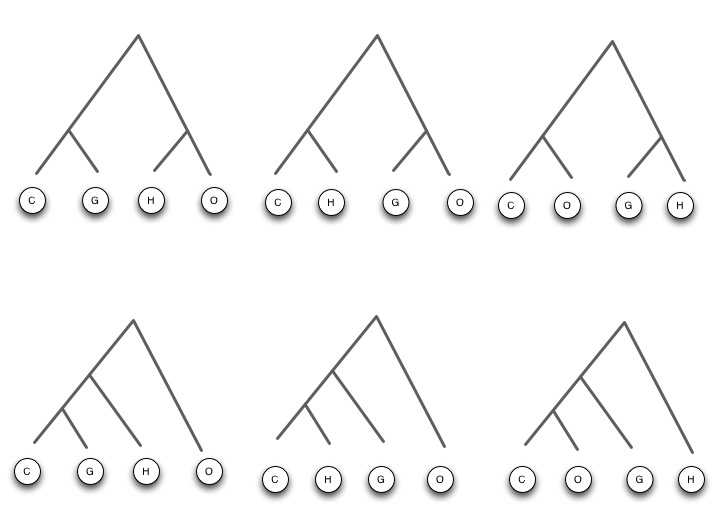
\includegraphics[width=5in]{trees.jpg}
	\end{center}
	\caption{Six binary tree topologies, utilizing two different tree structures.}
	\label{trees}
\end{figure}

\paragraph{b.}

I was only able to complete the Sankoff algorithm on one tree due to time constraints.  My results are shown in Figure~\ref{sankoff}.

\begin{figure}[htb]
	\begin{center}
		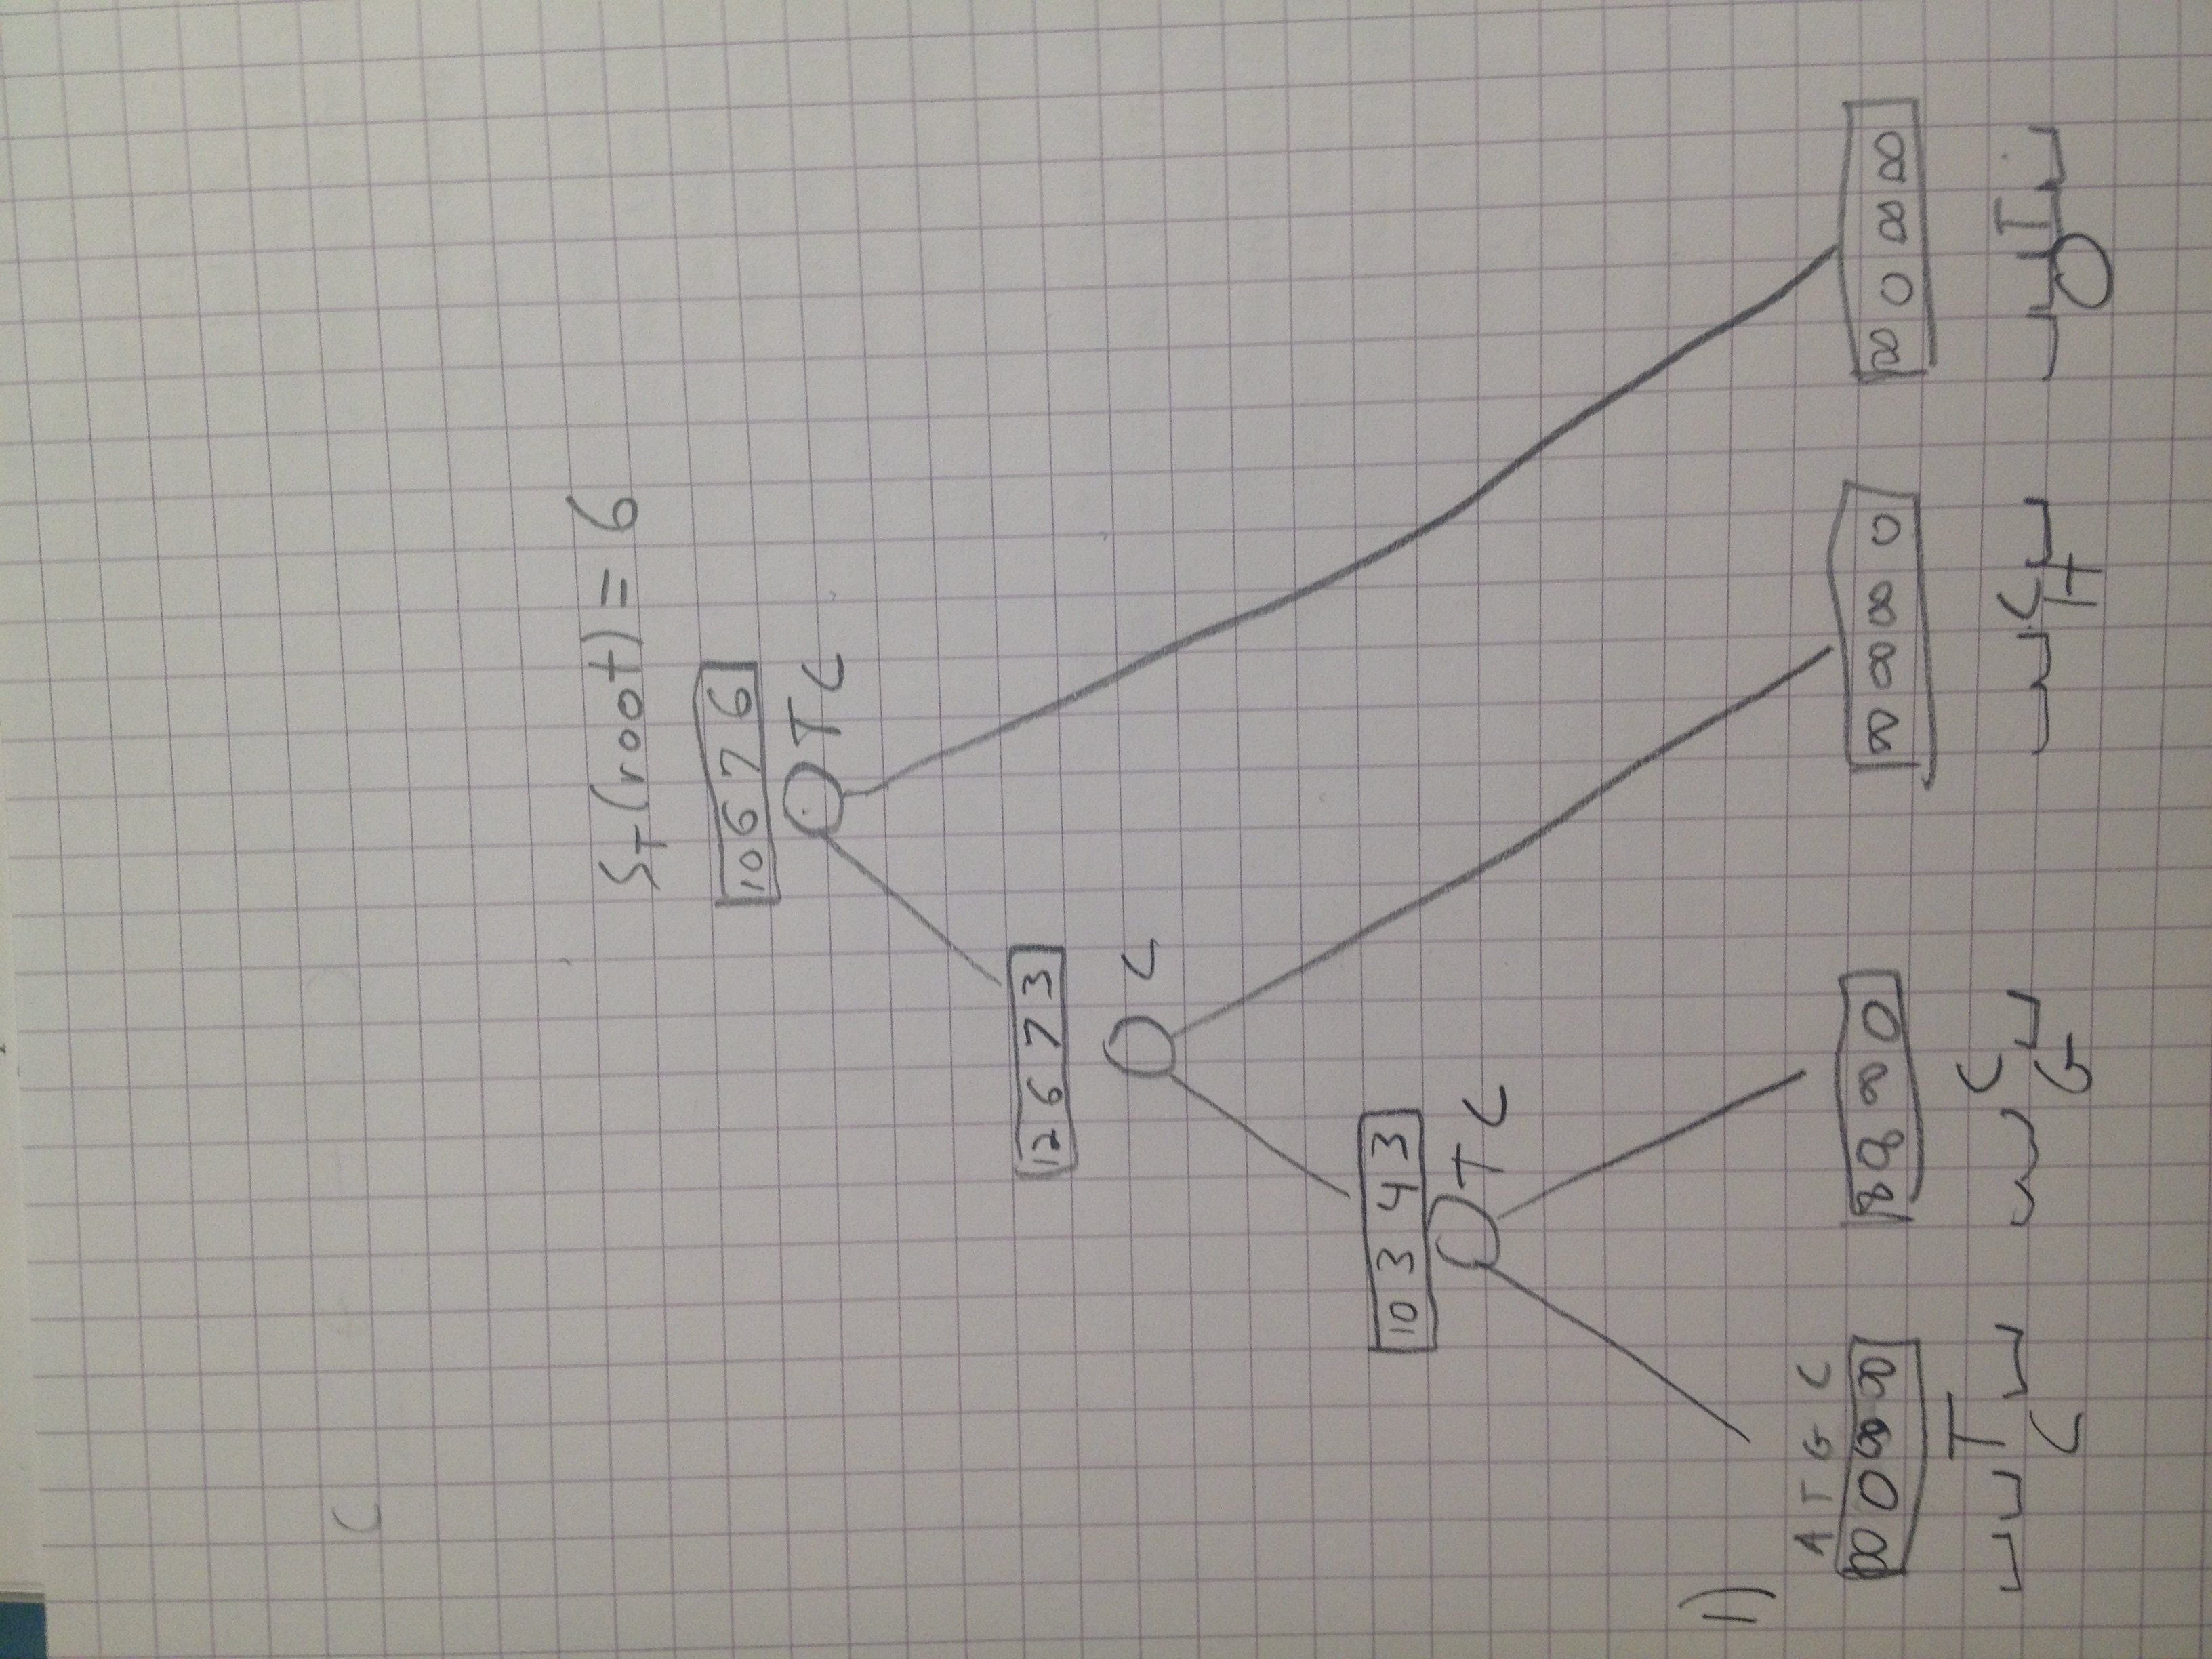
\includegraphics[width=3in, angle=-90]{sankoff.jpg}
	\end{center}
	\caption{The Sankoff algorithm applied to the topology in the lower left of Figure~\ref{trees}.}
	\label{sankoff}
\end{figure}

\paragraph{c.}

I was only able to complete the Fitch algorithm on one tree due to time constraints.  My results are shown in Figure~\ref{fitch}.

\begin{figure}[htb]
	\begin{center}
		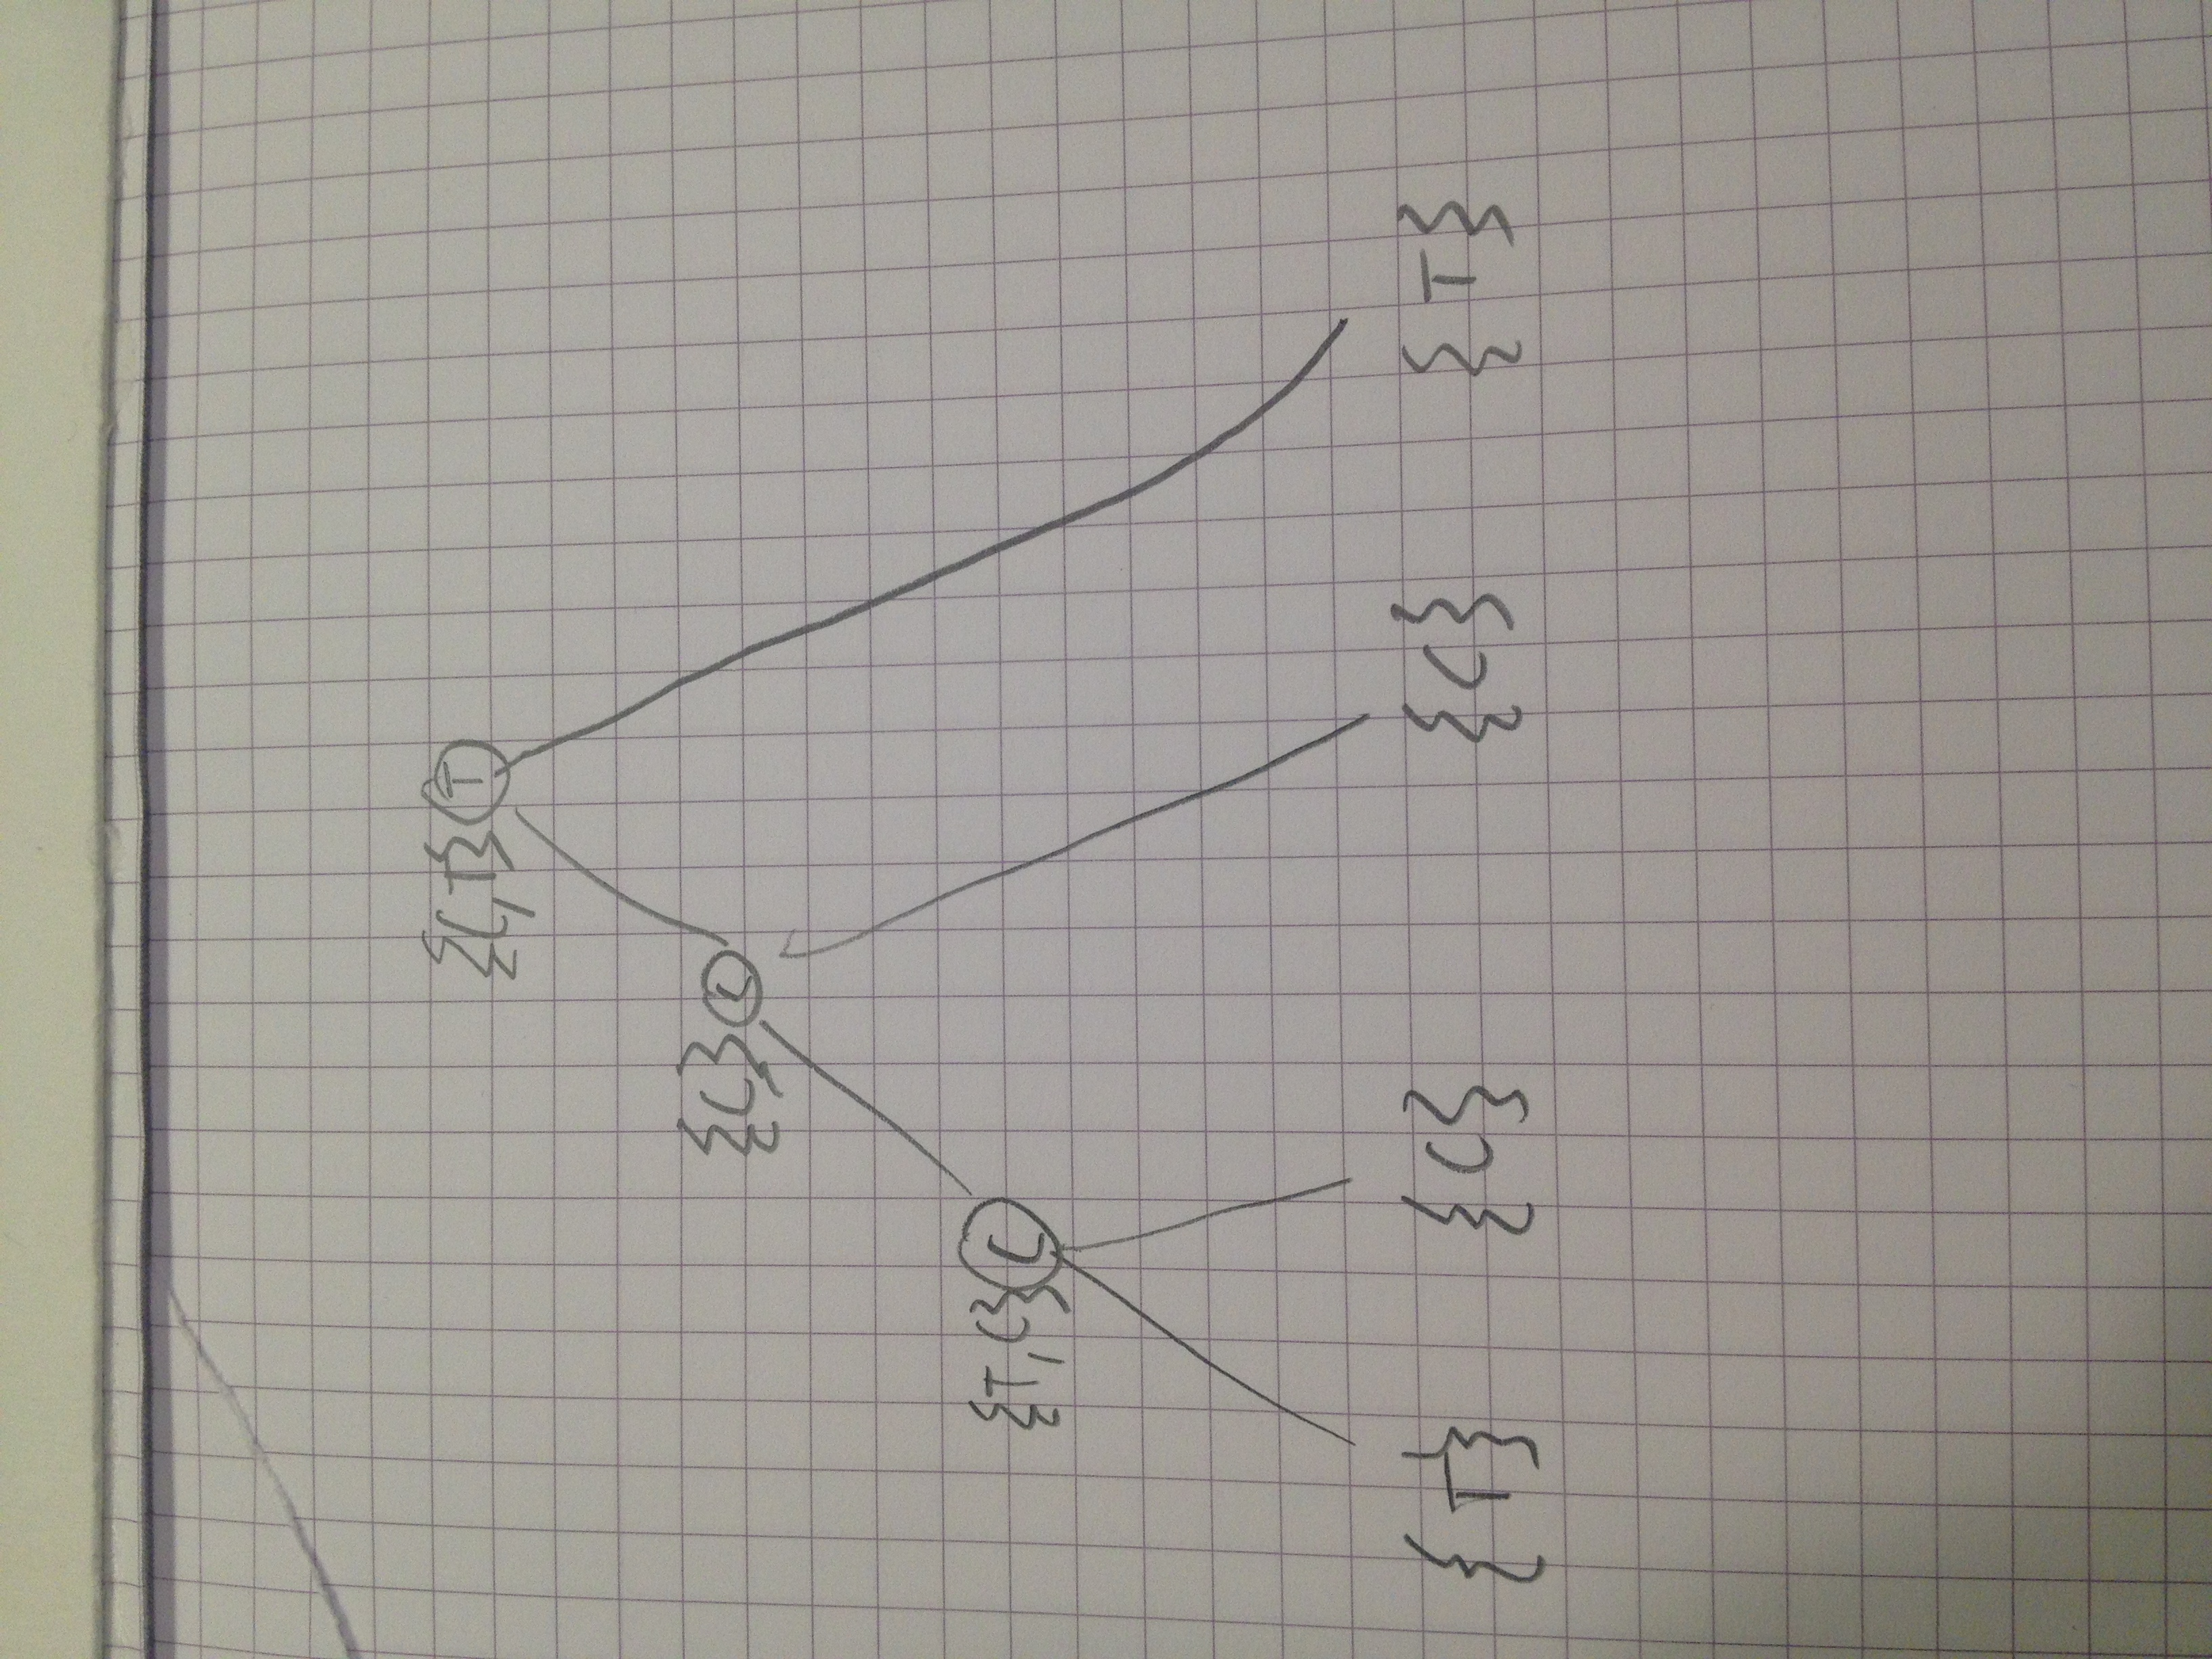
\includegraphics[width=3in, angle=-90]{fitch.jpg}
	\end{center}
	\caption{The Fitch algorithm applied to the topology in the lower left of Figure~\ref{trees}.}
	\label{fitch}
\end{figure}

\paragraph{d.} 

The algorithms produce identical results because they are algoithmic twins.  That is, the methods they use to calculate scores and assign vertex labels are computationally equivalent.

\clearpage
\section*{Question 2}
\paragraph{a.} 
A matrix is additive if there exists a tree $T$ with $d_{i,j}(T) = D_{i,j}$.  But an efficient way to determine this is the Four point theorem, which states that, for every combination of leaves $i$, $j$, $k$, and $l$, the sums $D_{i,j}, D_{j,k},$ and $ D_{k,l}$ yeild two identical sums, with the third sum smaller than these two.

To test this, I wrote a simple algorithm in Python.  It is shown in Figure~\ref{fourpoint}.  It confirms that every combinaion of  $i$, $j$, $k$, and $l$ satisfy the four point condition; the matrix is thus additive.

\begin{figure}[htb]
\centering
\begin{lstlisting}[language=Python]
def four_point():
# Determines whether a matrix is additive by testing for the four point condidtion.  Expects matrix as a list of lists

	n = len(matrix)

	for i in xrange(0,n):
		for j in xrange(0,n):
			if i == j:
				continue
			for k in xrange(0,n):
				if k == j:
					continue
				if k == i:
					continue
				for l in xrange(0,n):
					if l == k:
						continue
					if l == j:
						continue
					if l == i:
						continue
					one = matrix[i][j] + matrix[k][l]
					two = matrix[i][k] + matrix[j][l]
					three = matrix[i][l] + matrix[j][k]
					lump = sorted([one,two,three])
					if lump[1] != lump[2]:
						print "Not additive"
	\end{lstlisting}

	\caption{An algorithm to calculate whether the four point condition holds for an $n\times n$ matrix.}
	\label{fourpoint}


\end{figure}


\paragraph{b.} 
An efficient method for finding the $\delta$ for an interation is given by the pseudocode in Figure~\ref{finddelta}

\begin{figure}[htb]
\centering
\begin{lstlisting}
FindDelta(matrix)
	select any cell comtaining the minimum weight
	combine the leaves indicated (column, row) with another leaf
	connect all three leaves to a central node by edges $x, y, z$
	solve the following system:
		x + y = D(the nodes they connect)
		y + z = D(the nodes they connect)
		z + x = D(the nodes they connect)
	the minium of $x, y, z$ is the minium value of $\delta$
\end{lstlisting}
	\caption{An algorithm to to find the trimming parameter for additive tree reconstruction.}
	\label{finddelta}
\end{figure}

\paragraph{c.} % (fold)
Figure~\ref{twoiter} shows the $\delta$ and $i,j,k$ for the first two iterations on this matrix.

\begin{figure}[htb]
	\begin{center}
		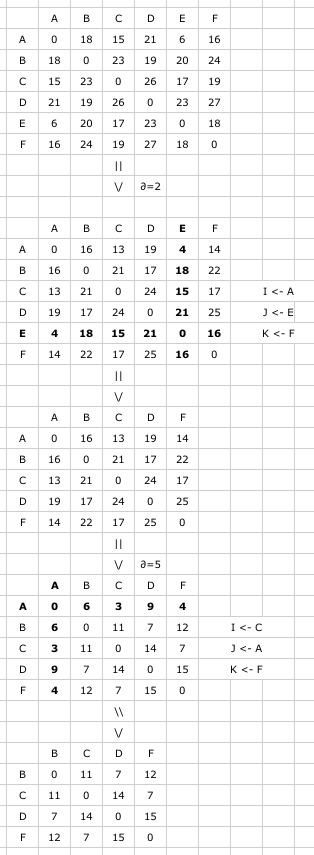
\includegraphics[width=2.25in]{twoiter}
	\end{center}
	\caption{The first two iterations of additive phylogenetic reconstruction.}
	\label{twoiter}
\end{figure}



\clearpage
\section*{Question 3}
For this problem let us define $i$ as the number of islands connected in a graph of arbitrary vertices. In this problem, $i=8$. Figure~\ref{twographs} shows an initial formulation of the boundaries of the problem of visiting each island.  On the left, the minumum possible trips are shown, which are $i-1 =7$.  On the right is an arrangement where the maximum number of trips must be taken.  Because of the inclusion of a central hub, many routes must be taken more than once.  In fact, were we not able to choose our starting island in this problem, this example would disprove the desired limit of 12 since the trip length is $((i-2)*2)-1=13$. \\
But the problem places no such restriction on us, and so the minumum number of trips in the pathological case is show in Figure~\ref{onegraph}, and is $((i-1)*2)-2=12$.  How can we prove that this is the maximum number of trips?  The graph shown on the right in Figure~\ref{twographs} and in Figure~\ref{onegraph} is pathological because there are the maximum amount of nodes connected by only one edge, 7, which is $i-1$, i.e. all nodes except the central node.  Each of these potentially requires two trips to visit and then keep visiting other islands, yielding $(i-1)*2=14$  But we know that all of the islands are visited before each vertex is traveled twice.  In fact, if one both starts and ends on one of the outlying islands as int he irght of Figure~\ref{onegraph}, two of these return trips can be eliminated, one each for the Start and End islands, giving us the answer of $((i-1)*2)-2=12$.  Starting on the central island, as in the right of Figure~\ref{twographs} eliminates only one of these return trips, yielding $((i-1)*2)-1=13$.

\begin{figure}[htb]
	\begin{center}
		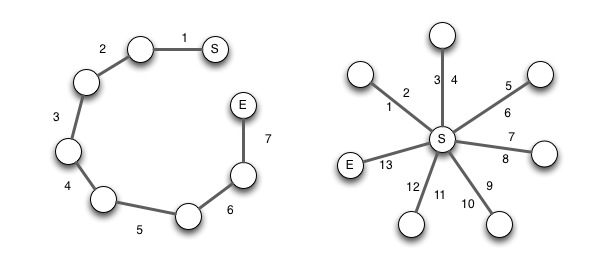
\includegraphics[width=4.5in]{twographs.jpg}
	\end{center}
	\caption{Initial formulation of the problem.  The tree on the left shows the minimum trips possible to visit all islands (i, while the tree on the right shows the pathological case where the maximum amount of trips must be taken if the starting islands cannot be chosen.  Start and end positions are marked by S and E, respectively, and trips are numbered.}
	\label{twographs}
\end{figure}


\begin{figure}[htb]
	\begin{center}
		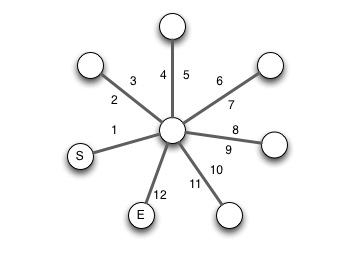
\includegraphics[width=3in]{onegraph.jpg}
	\end{center}
	\caption{The shortest path visiting all islands in the pathological case, where the starting islands are able to be chosen.  Its length is $(i-1)*2 - 2 = 12$}
	\label{onegraph}
\end{figure}

\clearpage

\section*{Question 4}
\paragraph{a}  The hidden markov model for this problem is in Figure~\ref{hmm}

\begin{figure}[htb]
	\begin{center}
		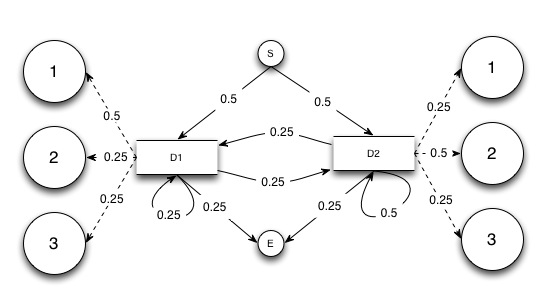
\includegraphics[width=4.5in]{hmm.jpg}
	\end{center}
	\caption{A hidden markov model of $Q=\textit{start},D1,D2,\textit{end}$ and $\Sigma = 1,2,3$}
	\label{hmm}
\end{figure}

\paragraph{b} % 1 1 2 1 2 2 

Table~\ref{viterbi} shows a Viterbi table for this sequence.  A sequnce that would satisfy this table is
\begin{align*}
	D_1, D_1, D_1, D_1, D_2, D_2, End
\end{align*}

The probability of this particular sequence 

\begin{table}[tb]
	\centering
	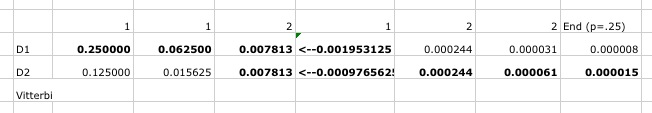
\includegraphics[width=5in]{./viterbi.jpg}
	\caption{The Viterbi table for problem 4.  The arrows are implicit for most of the table, pointing towards cells in bold; in the two ambiguous cases arrows are indicated, showing two possible paths.}
	\label{viterbi}
\end{table}



\paragraph{c} 
The second sequence of states implied by Table~\ref{viterbi} is
\[
	D_1, D_1, D_2, D_2, D_2, D_2, End
\]

The probability of this sequence occuring, independent of the emisions above, is given by
$$\begin{array}{cccccccccccccccccccc}
	\text{start}& &D_1& &D_1& &D_2& &D_2& &D_2& &D_2& &\text{end}&\\
	&.5&\cdot&.5&\cdot&.5&\cdot&.25&\cdot&.5&\cdot&.5&\cdot&.5&\cdot&.25&= 0.0009765\\
\end{array}$$
\section*{Question 5}
The probability that state $k$ caused emission $x$ at moment $i$ is given by
\[
	 P(\pi_i = k|x) = \frac{f_{k}(i) \cdot b_k(i)}{P(x|\pi)}
\]
Also,
\[
	f_{k}(i) = e_k(x_i)\cdot \sum_{l\in Q} f_{l,i-1}\cdot a_{l,k} 
\]
and
\[
	b_{k}(i) = e_k(x_i)\cdot \prod_{l\in Q} f_{l,i-1}\cdot a_{l,k}
\]
Finally,
\[
	P(x)=\sum_\pi P(x|\pi)
\]
I calculate these three terms, respectively, as
\begin{align*}
	f_{D_1}(x_4)=& 0.005127 \\
	b_{D_1}(x_4)=& 0.017578\\
	P(x) =& 0.000159
\end{align*}
This yields  % ############# need real numbers here.
\[
	P(\pi_i = k|x) = \frac{0.005127 \cdot 0.017578}{0.000159} = 0.566807
\]

This means that there's greater than 56\% chance that the dealer rolled the third 1 from $D_1$.  This makes intuitive sense: there are only two choices at that point, and the calculations I have slightly favor $D_1$ at that roll.  The tables I used for these calculations are shown in Table~\ref{fbcalcs}.

\begin{table}[hbt]
	\begin{center}
		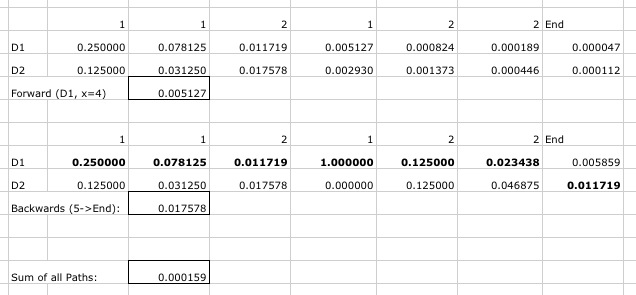
\includegraphics[width=5in]{fbcalcs.jpg}
	\end{center}
	\caption{Supporting calculations for $f_{D_1}(x_4),b_{D_1}(x_4),$ and $P(x)$ }
	\label{fbcalcs}
\end{table}

\end{document}
